\documentclass[border=10pt,tikz,convert]{standalone}

% Requigray package
\usetikzlibrary{shapes, arrows.meta, positioning}
\usetikzlibrary{shadows}

\let\svtikzpicture\tikzpicture
\def\tikzpicture{\noindent\svtikzpicture}

\newlength{\w}
\setlength{\w}{4cm}

\newlength{\h}
\setlength{\h}{1.25cm}

\newlength{\s}
\setlength{\s}{3cm}

%\definecolor{outcolor}{rgb}{0.73, 0.33, 0.83}    % medium orchid
%\definecolor{incolor}{rgb}{0.85, 0.57, 0.0}			 % harvest gold
%\definecolor{hiddencolor}{rgb}{0.28, 0.82, 0.8} % medium turquoise


%\definecolor{outcolor}{rgb}{0.84, 0.32, 0.03}    % medium orchid
%\definecolor{outcolor}{rgb}{0.60, 0.37, 0.60}
%\definecolor{incolor}{rgb}{0.94, 0.63, 0.04}			 % harvest gold
%\definecolor{hiddencolor}{rgb}{0.33, 0.87, 0.88} % medium turquoise


\definecolor{outcolor}{rgb}{0.55, 0.0, 0.55}
\definecolor{hiddencolor}{rgb}{0.19, 0.55, 0.91}
\definecolor{incolor}{rgb}{0.0, 0.55, 0.55} % purple
%\definecolor{incolor}{rgb}{0.91, 0.41, 0.17} % orange

\definecolor{bgcolor}{rgb}{0.74, 0.83, 0.9}   % gray-blue



\tikzset{input/.style={draw=incolor!30, fill=incolor!30, text=incolor!20!black, minimum width=\w, minimum height=1cm,drop shadow}}
\tikzset{hidden/.style={draw=hiddencolor!30, fill=hiddencolor!30, text=hiddencolor!20!black, minimum width=\w, minimum height=1cm,drop shadow}}
\tikzset{output/.style={draw=outcolor!30, fill=outcolor!30, text=outcolor!20!black, minimum width=\w, minimum height=1cm,drop shadow}}

\begin{document}


	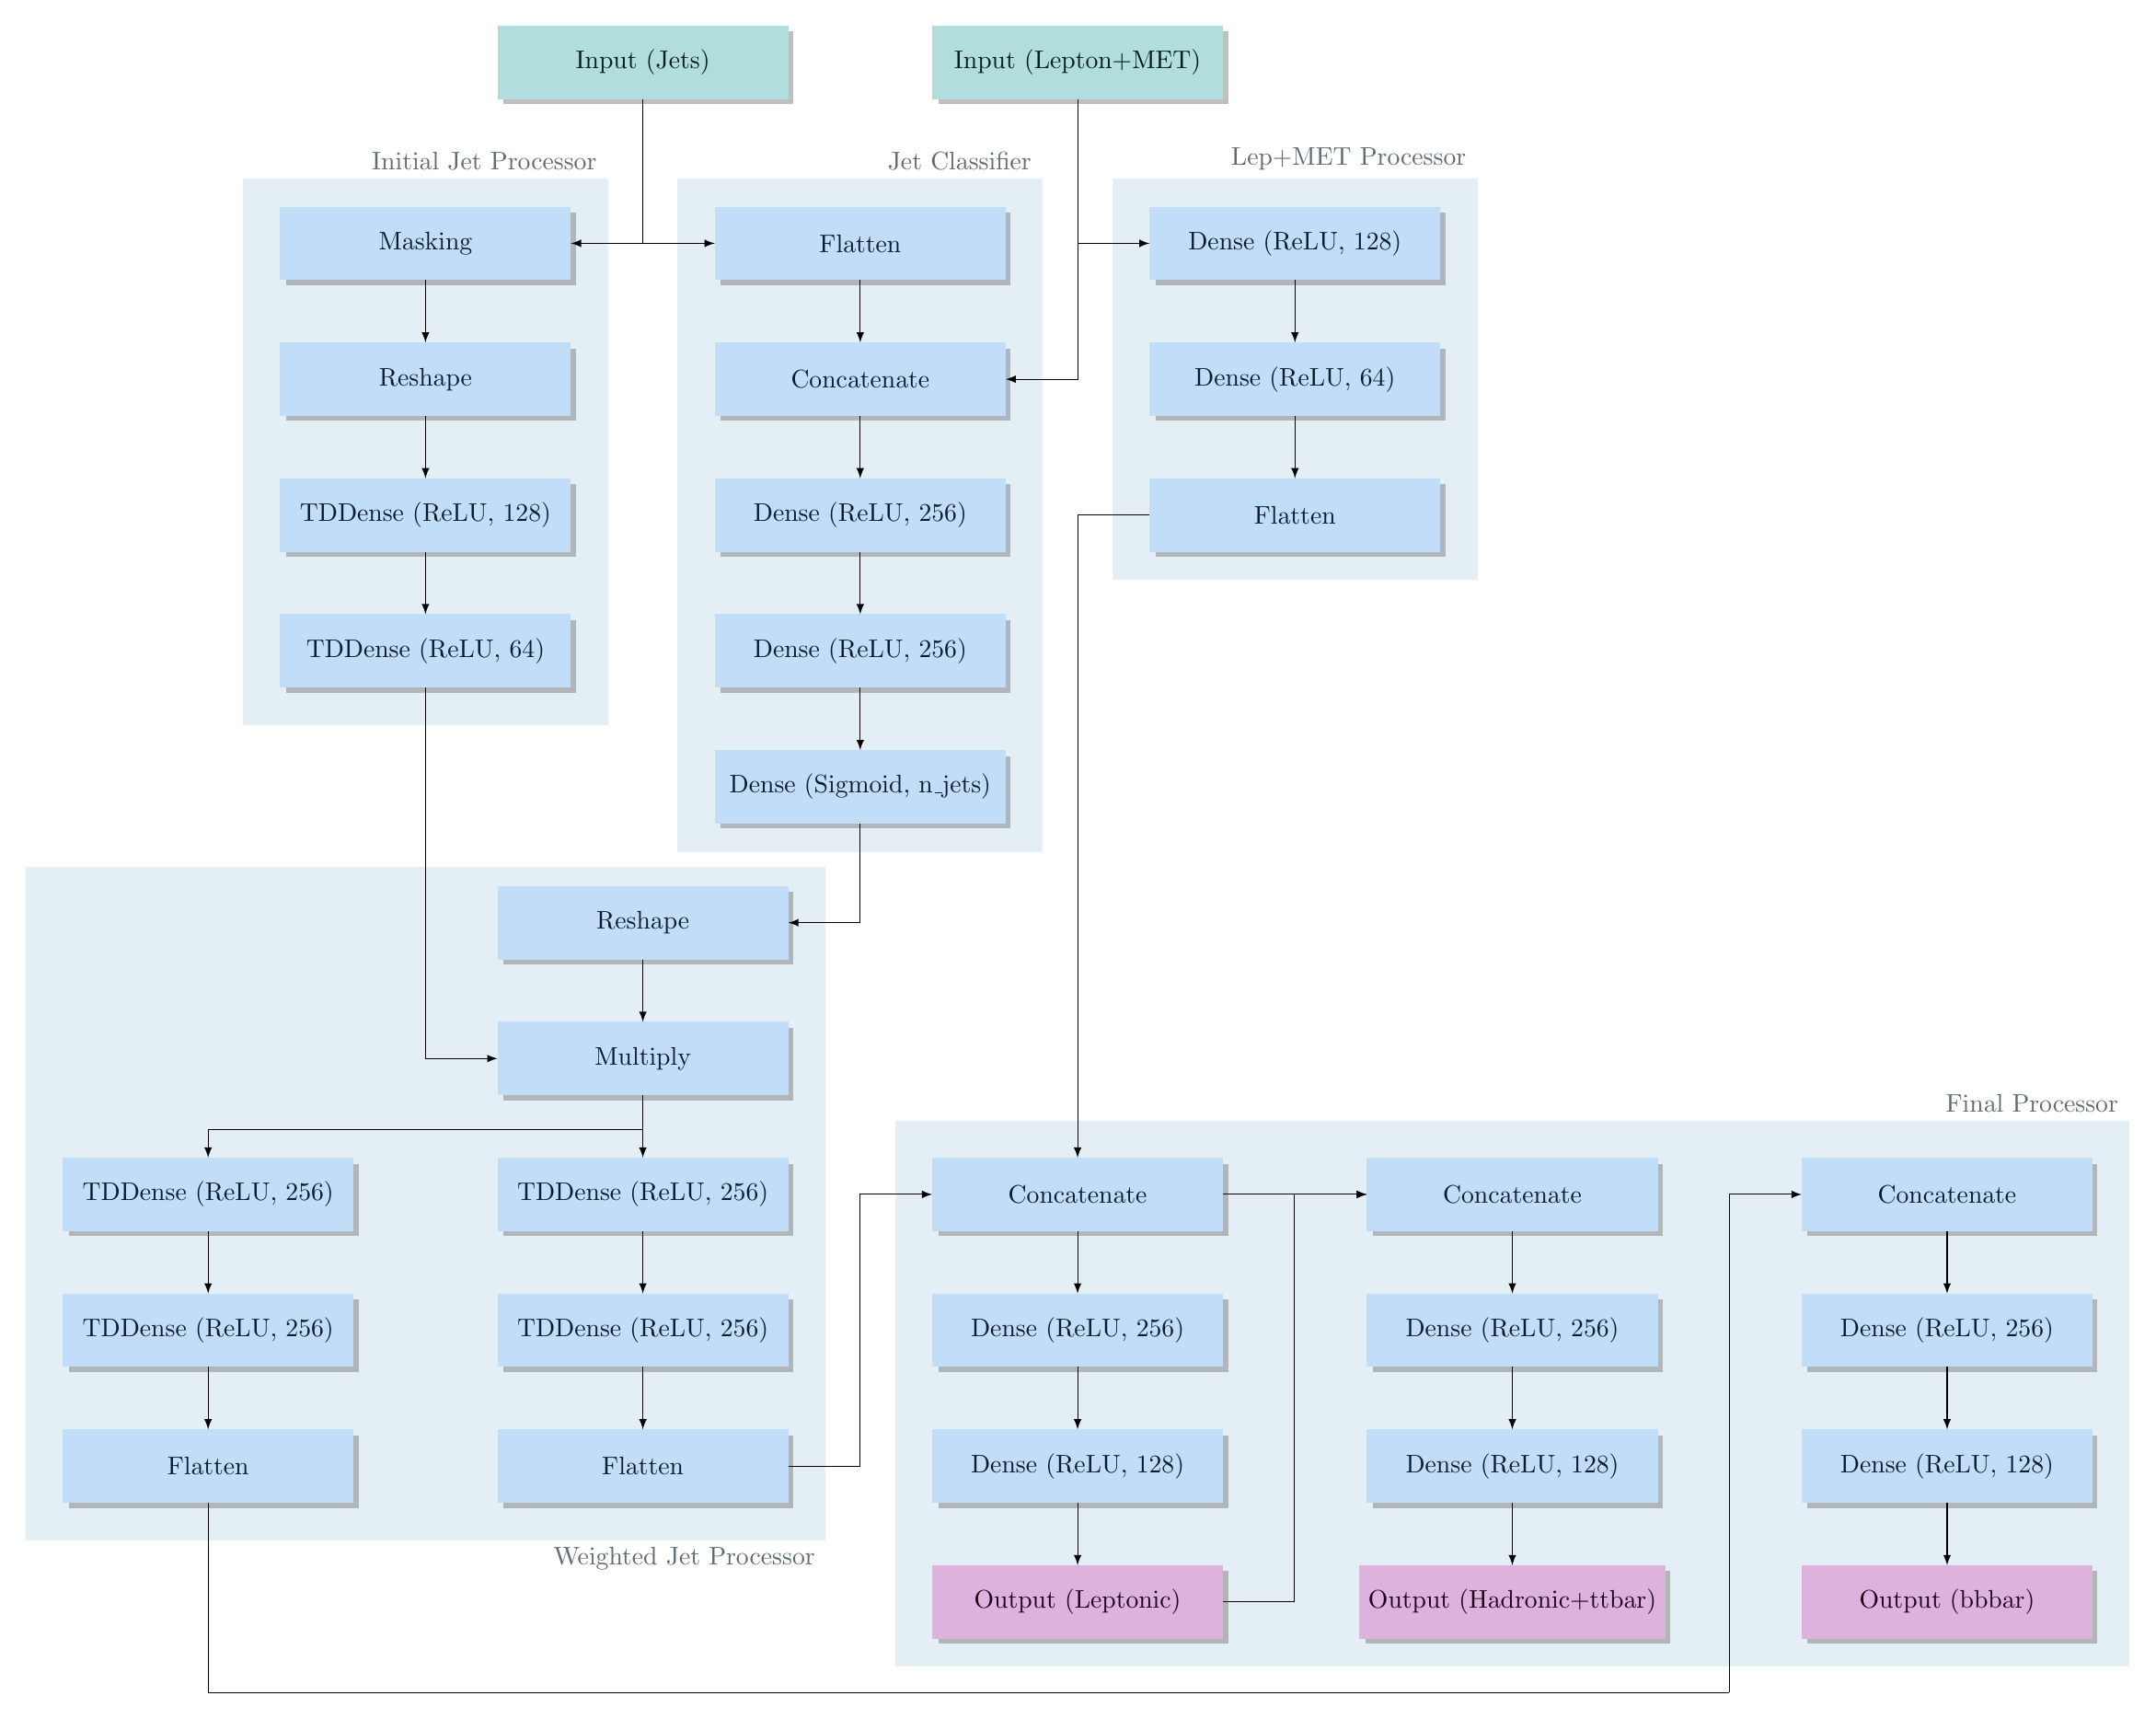
\begin{tikzpicture}
	
	%%% NODES %%%
	
	
	% INPUTS
	\node[input] at (\s,0.5*\h) (jetinput) {Input (Jets)};
	\node[input] at (3*\s,0.5*\h) (otherinput) {Input (Lepton+MET)};
	
	% JET PRETRAINER
	\draw[draw=bgcolor!40,very thick,fill=bgcolor!40] (8.5,-1) node[above left,color=bgcolor!50!black] {Jet Classifier} rectangle ++(-5,-9.25);
	\node[hidden] at (2\s,-1.5*\h) (flattenedjets) {Flatten};
	\node[hidden] at (2\s,-3*\h) (concatjetsother) {Concatenate};
	\node[hidden] at (2\s,-4.5*\h) (dense256-1) {Dense (ReLU, 256)};
	\node[hidden] at (2\s,-6*\h) (dense256-2) {Dense (ReLU, 256)};
	\node[hidden] at (2\s,-7.5*\h) (jetmatchoutput) {Dense (Sigmoid, n\_jets)};
	
	
	% JET PATH
	\draw[draw=bgcolor!40,very thick,fill=bgcolor!40] (2.5,-1) node[above left,color=bgcolor!50!black] {Initial Jet Processor} rectangle ++(-5,-7.5);
	\node[hidden] at (0,-1.5*\h) (maskingjets) {Masking};
	\node[hidden] at (0,-3*\h) (reshapemaskedjets) {Reshape};
	\node[hidden] at (0,-4.5*\h) (TDDense128) {TDDense (ReLU, 128)};
	\node[hidden] at (0,-6*\h) (TDDense64) {TDDense (ReLU, 64)};
	
	% OTHER PATH
	\draw[draw=bgcolor!40,very thick,fill=bgcolor!40] (14.5,-1) node[above left,color=bgcolor!50!black] {Lep+MET Processor} rectangle ++(-5,-5.5);
	\node[hidden] at (4*\s,-1.5*\h) (dense128) {Dense (ReLU, 128)};
	\node[hidden] at (4*\s,-3*\h) (dense64) {Dense (ReLU, 64)};
	\node[hidden] at (4*\s,-4.5*\h) (flattenedother) {Flatten};
	
	% JET REWEIGHTING
	\draw[draw=bgcolor!40,very thick,fill=bgcolor!40] (5.5,-10.5) rectangle ++(-11,-9.25) ;
	\node[below left, color=bgcolor!50!black] at (5.5,-19.75) {Weighted Jet Processor};
	\node[hidden] at (\s,-9*\h) (reshape) {Reshape};
	\node[hidden] at (\s,-10.5*\h) (weightjets) {Multiply};
	\node[hidden] at (\s,-12*\h) (TDDense256-1) {TDDense (ReLU, 256)};
	\node[hidden] at (\s,-13.5*\h) (TDDense256-2) {TDDense (ReLU, 256)};
	\node[hidden] at (\s,-15*\h) (flattenedweightedjets) {Flatten};
	
	\node[hidden] at (-\s,-12*\h) (TDDense256-1-2) {TDDense (ReLU, 256)};
	\node[hidden] at (-\s,-13.5*\h) (TDDense256-2-2) {TDDense (ReLU, 256)};
	\node[hidden] at (-\s,-15*\h) (flattenedweightedjets-2) {Flatten};
	
	% FIRST ENDING (LEP)
	\draw[draw=bgcolor!40,very thick,fill=bgcolor!40] (23.5,-14) node[above left,color=bgcolor!50!black] {Final Processor} rectangle ++(-17,-7.5);
	\node[hidden] at (3*\s,-12*\h) (concateverything) {Concatenate};
	\node[hidden] at (3*\s,-13.5*\h) (ldense256) {Dense (ReLU, 256)};
	\node[hidden] at (3*\s,-15*\h) (ldense128) {Dense (ReLU, 128)};
	\node[output] at (3*\s,-16.5*\h) (lepoutput) {Output (Leptonic)};
	
	% SECOND ENDING (HAD)
	\node[hidden] at (5*\s,-12*\h) (hconcat) {Concatenate};
	\node[hidden] at (5*\s,-13.5*\h) (hdense256) {Dense (ReLU, 256)};
	\node[hidden] at (5*\s,-15*\h) (hdense128) {Dense (ReLU, 128)};
	\node[output] at (5*\s,-16.5*\h) (hadoutput) {Output (Hadronic+ttbar)};
	
	% THIRD ENDING (BB)
	\node[hidden] at (7*\s,-12*\h) (bconcat) {Concatenate};
	\node[hidden] at (7*\s,-13.5*\h) (bdense256) {Dense (ReLU, 256)};
	\node[hidden] at (7*\s,-15*\h) (bdense128) {Dense (ReLU, 128)};
	\node[output] at (7*\s,-16.5*\h) (boutput) {Output (bbbar)};
	
	
	
	
	
	%%% EXTRA ARROW NODES %%%
	\node[coordinate, below=0.375*\h of weightjets] (e0) {};
	\node[coordinate, left=0.25*\w of concateverything] (e1) {};
	\node[coordinate, left=0.25*\w of hconcat] (e2) {};
	\node[coordinate, left=0.25*\w of bconcat] (e3) {};
	\node[coordinate, below=3*\h of e1] (e4) {};
	\node[coordinate, below= 5.5*\h of e3] (e5) {};
	\node[coordinate, below= 5.5*\h of e2] (e6) {};
	
	
	
	
	%%% ARROWS %%%
	
	% JET PRETRAINER
	\draw[-latex] (jetinput) |- (flattenedjets);
	\draw[-latex] (flattenedjets) -- (concatjetsother);
	\draw[-latex] (otherinput) |- (concatjetsother);
	\draw[-latex] (concatjetsother) -- (dense256-1);
	\draw[-latex] (dense256-1) -- (dense256-2);
	\draw[-latex] (dense256-2) -- (jetmatchoutput);
	\draw[-latex] (jetmatchoutput) |- (reshape);
	
	% JET PATH
	\draw[-latex] (jetinput) |- (maskingjets);
	\draw[-latex] (maskingjets) -- (reshapemaskedjets);
	\draw[-latex] (reshapemaskedjets) -- (TDDense128);
	\draw[-latex] (TDDense128) -- (TDDense64);
	
	% OTHER PATH
	\draw[-latex] (otherinput) |- (dense128);
	\draw[-latex] (dense128) -- (dense64);
	\draw[-latex] (dense64) -- (flattenedother);
	
	% JET REWEIGHTING
	\draw[-latex] (reshape) -- (weightjets);
	\draw[-latex] (TDDense64) |- (weightjets);
	\draw[-latex] (weightjets) -- (TDDense256-1);
	\draw[-latex] (TDDense256-1) -- (TDDense256-2);
	\draw[-latex] (TDDense256-2) -- (flattenedweightedjets);
	\draw (weightjets) -- (e0);
	\draw[-latex] (e0) -| (TDDense256-1-2);
	\draw[-latex] (TDDense256-1-2) -- (TDDense256-2-2);
	\draw[-latex] (TDDense256-2-2) -- (flattenedweightedjets-2);
	\draw (flattenedweightedjets-2) |- (e5); 
	
	% FIRST ENDING
	\draw (flattenedweightedjets) -| (e1);
	\draw[-latex] (e1) -- (concateverything);
	\draw[-latex] (flattenedother) -| (concateverything);
	\draw[-latex] (concateverything) -- (ldense256);
	\draw[-latex] (ldense256) -- (ldense128);
	\draw[-latex] (ldense128) -- (lepoutput);
	
	% SECOND ENDING
	\draw (lepoutput) -| (e2);
	\draw[-latex] (e2) -- (hconcat);
	\draw[-latex] (concateverything) -- (hconcat);
	\draw[-latex] (hconcat) -- (hdense256);
	\draw[-latex] (hdense256) -- (hdense128);
	\draw[-latex] (hdense128) -- (hadoutput);
	
	% THIRD ENDING
	\draw (e5) -- (e3);
    \draw[-latex] (e3) -- (bconcat);
	\draw[-latex] (bconcat) -- (bdense256);
	\draw[-latex] (bdense256) -- (bdense128);
	\draw[-latex] (bdense128) -- (boutput);
	
\end{tikzpicture}

\end{document}